\RequirePackage[l2tabu, orthodox]{nag} % Warn about outdated commands/packages.
% The report class uses some outdated commands, about which nag will complain.
% You can just ignore these warnings.

\documentclass[11pt, a4paper]{report} % Sets font and paper size.

%%% General formatting packages (order is important, so don't sort) %%%
\usepackage{amsmath} % More equation formatting.
\usepackage[dutch, english]{babel} % Language specific quirks.
\usepackage{booktabs} % Improved tables.
\usepackage[font=small]{caption} % Better caption formatting.
\usepackage{fancyhdr} % Modification of headers and footers.
\usepackage[T1]{fontenc} % Makes one unicode character of special input (e.g. ö).
\usepackage[margin=1.25in]{geometry} % Control page layout.
\usepackage{float} % More control over image positions.
\usepackage{graphicx} % Include graphics. Use '\graphicspath' to locate files in a different folder.
\usepackage[utf8]{inputenc} % Special characters (e.g. trema) can be entered directly: .tex file has to be saved using UTF-8 encoding.
\usepackage{lmodern} % Alternative font because 'fontenc' package does not work with default.
\usepackage{microtype} % Improves character spacing.
\usepackage[sort]{natbib} % Provides (author, year) references. \citet: textual, \citep: parenthetical
\usepackage{physics} % Provides physics macros such as Dirac notation.
\usepackage{tikz} % Draw diagrams and figures.
\usepackage{url} % Allow inclusion of urls in text.
\usepackage{siunitx} % SI unit formatting and scientific notation.
\usepackage{subcaption} % Allow subcaptions.
\usepackage[nottoc]{tocbibind} % Include references in table of contents.
\usepackage[colorinlistoftodos]{todonotes} % Add todo notes.
\usepackage{varioref} % Automatically put reference to page in reference. Use \vref.
\usepackage{cleveref} % Automate "equation (...)" reference. Use \vref.
\usepackage{commath}
\usepackage{breqn}

%%% Additional options %%%
\pagestyle{fancy} % Set header style.
\setlength{\headheight}{14pt}
\fancyhead[R]{\rightmark}
\fancyhead[L]{}


%%% Personal Information %%%
\newcommand\TITLE{Monte Carlo Simulations of the 3-State Potts Model in 2D}
\newcommand\THESISFORM{Bachelor Project Physics and Astronomy, size 15 EC\\conducted between 29-03-2016 and xx-xx-2016}
\newcommand\INSTITUTE{Instituut voor Theoretische Fysica Amsterdam}
\newcommand\FACULTY{Faculteit der Natuurwetenschappen, Wiskunde en Informatice}
\newcommand\UNIVERSITY{Universiteit van Amsterdam}
\newcommand\AUTHOR{Teun Zwart (10499873)}
\newcommand\SUPERVISOR{dr. Phillipe Corboz}
\newcommand\SECONDASSESSOR{dr. Edan Lerner}
\newcommand\UNIVERSITYLOGO{UvA-logo.png} % Uncomment line below and add name of logo file.

\graphicspath{{./images/}}


\begin{document}

\begin{titlepage}
	\begin{center}
		\rule{\textwidth}{0.4mm}\\[0.5cm]
		\huge{\textbf{\TITLE}}
		\rule{\textwidth}{0.4mm}\\[0.5cm]
		\large{\THESISFORM}\\[0.5cm]
		\begin{minipage}[t]{0.4\textwidth}
			\begin{flushleft}
				\large\emph{Author}\\{\AUTHOR}
			\end{flushleft}
		\end{minipage}
		\begin{minipage}[t]{0.4\textwidth}
			\begin{flushright}
				\large\emph{Supervisor}\\{\SUPERVISOR}\\~\\
				\large\emph{Second Assessor}\\{\SECONDASSESSOR}
			\end{flushright}
		\end{minipage}
		\vfill
		\large{\INSTITUTE}\\
		\large{\FACULTY}\\
		\large{\UNIVERSITY}\\~\\
		\includegraphics[width=1.5cm]{\UNIVERSITYLOGO}
	\end{center}
\end{titlepage}

\thispagestyle{plain}
\section*{Abstract}


\newpage
\thispagestyle{plain}
\section*{Populaire Samenvatting}


\tableofcontents

\chapter{Introduction}

\chapter{Models and Critical Phenomena}

\section{Phase Transitions and Critical Phenomena}
Phase transitions are an everyday part of life, the most well known being the transition of water into water vapor or ice into water.
To determine when a phase transition has taken place, we consider the order parameter.
In ferromagnetic systems such as iron, as well as in the systems we will study in this work, this is the magnetization.
On one side of the phase transition a non-zero magnetization is present.
As the iron is heated, it moves past its Curie temperature and the magnetization does become zero.
More generally we consider an order parameter \(\phi\) which is a quantity that is non-zero on one side of the phase transition, and vanished on the other side. Usually the order parameter is zero on the high temperature side of the phase transition. (See \cref{fig:ising_magnetization}. The Ising model is considered in more detail in \cref{sec:ising_model}.)
The temperature at which the order parameter becomes zero is the critical temperature \(T_c\).
\begin{figure}[h]
	\centering
	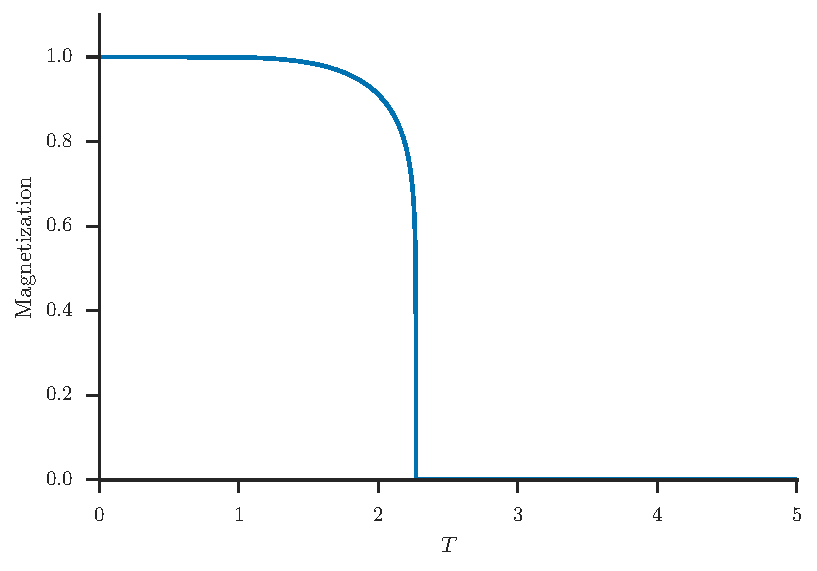
\includegraphics[width=0.66\textwidth]{ising_magnetization}
	\caption{The magnetization of the two-dimensional Ising model. Notice how the magnetization is finite on one side of the phase transition, but zero on the other side.}
	\label{fig:ising_magnetization}
\end{figure}

When we consider phase transitions, we distinguish two different kinds.
The phase transition associated with freezing water is what is called first-order.
As the critical temperature is crossed the water molecules move from a disordered phase into an ordered crystal phase.
As this happens, energy is emmited in the form of latent heat.
This is defined as
\begin{equation}
	\label{eq:laten_heat}
	l = \int_{T_c-}^{T_c+} c(T) \dif T,
\end{equation}
with \(l\) the latent heat and \(c(T)\) the heat capacity of the system.
In first order transition the order parameter is discontinous at \(T_c\).\cite{binney:1992}
In the rest of this work we only consider second-order transitions, for which the latent heat is zero and the order parameter, but not the rate of change of the order parameter is continuous at \(T_c\).

While the latent heat of a transition may be zero, this need not be the case for the heat capacity of the system or other thermodynamic properties such as the magnetic susceptibility.
Often the heat capacity diverces as \(c \propto \abs{T-T_c}^{-\alpha}\).
We call \(\alpha\) a critical exponent.
Because for continuous phase transitions the latent heat has to vanish by definition, \(\alpha\) has to be smaller than 1, because otherwise the integral of \cref{eq:latent_heat} diverges.
No divergence occurs if \(\alpha < 0\).
In the limiting case that \(\alpha = 0\), we can consider the divergence of the specific heat to be logarithmic since
\begin{equation}
	\log(\frac{1}{x}) = \lim_{\alpha \to 0+} \frac{1}{\alpha}\left(x^{-\alpha} - 1\right).
\end{equation}
Theoretically and experimentally we find that the exponent governing divergence is the same both above and below \(T_c\).\cite{binney:1992}

\subsection{Correlation Functions}
For the systems we would like to consider it is often interesting to quantify how different parts of system relate to each other.
In fact we will see that this correlation proves critical when choosing an appropriate algorithm to numerically study systems around the critical temperature (\cref{sec:critical_slowing_down}).
To quantify the correlations in a system we define the two-point correlation function\cite{binney:1992}, which, to illustrate some properties of the correlation function, we first define for a system of spins:
\begin{equation}
	G^{(2)}(\mathbf{i}, \mathbf{j}) = \langle{\mathbf{s}_i \cdot \mathbf{s}_j}\rangle.
\end{equation}
Here \(\mathbf{i}\) and \(\mathbf{j}\) are the position vectors of the spins at locations \(i\) and \(j\) respectively.
The angle brackets denote thermal averaging.
Because the system is often translationally invariant as well as isotropic, meaning it has no preferred direction, such as in a crystal lattice or in disordered systems, \(G^{(2)}\) often depends only on \(\abs{\mathbf{i} - \mathbf{j}} \)

In the general case the two-point correlation function is defined as
\begin{equation}
	G^{(2)}(r) = \langle \boldsymbol{\phi}(0) \cdot \boldsymbol{\phi}(\mathbf{r}) \rangle,
\end{equation}
where \(\phi\) is the order parameter of the system.
Below \(T_c\) the system is ordered and \(G^{(2)}\) is large for all \(r\).
In the example using spins given above, this means almost all spins are aligned.
A more useful quantity in this case is the connected correlation function
\begin{equation}
	G_c^{(2)} = \langle \boldsymbol{\phi}(0) \cdot \boldsymbol{\phi}(\mathbf{r}) \rangle - \abs{\langle \phi \rangle}^2.
\end{equation}
By subtracting the thermally averaged value of the order parameter from the two-point correlation function, we can ignore the general alignment of the order parameter and only have fluctuations in the order parameter contribute.

When \(T/T_c\) is either large or small \(G_c^{(2)}\) is small.
Precisely at the critical temperature \(G_c^{(2)}\) has the form
\begin{equation}
	G_c^{(2)} \propto \frac{1}{r^{d-2+\eta}},
\end{equation}
with \(d\) the dimensionality of the system and \(\eta\) another critical exponent.
Far away from \(T_c\) \(G_c^{(2)}\) can not be approximated by a power law, but for \(\abs{T-T_c} / T_c \ll 1\) \(G_c^{(2)}\) has the form
\begin{equation}
	G_c^{(2)} \propto \frac{e^{-r/\xi}}{r^{d-2+\eta}}.
\end{equation}
\(\xi\) denotes the correlation length.
Fluctuations of the order parameter up to this length scale are common, but larger fluctuations are exponentially suppressed.
The correlation length diverges as \(T_c\) is approached from above or below, according to
\begin{equation}
	\xi \propto \abs{T-T_c}^{-\nu},
\end{equation}
where \(\nu\) is another critical exponent.

\subsection{Scaling Laws}
We can define three other critical exponents.
For the magnetic susceptibility we have
\begin{equation}
	\chi \propto \abs{T-T_c}^{-\gamma},
\end{equation}
while for the magnetization of a system we have
\begin{equation}
	m \propto \abs{T-T_c}^{\beta} \mathrm{\ \ \ \ \ T \to T_c\ from\ below}.
\end{equation}
Finally we can define a critical exponent for the magnetization in a non-zero magnetic field (the previous five critical exponents assumed \(B=0\)).
Precicesly at \(T_c\)
\begin{equation}
	m \propto B^{1/\delta} \mathrm{\ \ \ \ \ B \to 0}.
\end{equation}

These six critical exponents are not independent of each other but are related through scaling laws.
Given these scaling laws only two critical exponents need to be known to determine all others as well.
They are:
\begin{align}
	\alpha + 2\beta +\gamma &= 2\\
	\alpha + \beta(\delta+1) &= 2\\
	(2-\eta)\nu &= \gamma \\
	\nu d &= 2- \alpha,
\end{align}
with \(\nu\) the dimensionalty of the system.\cite{binney:1992,baxter:1973,landau:2015}\todo{Put some part of the derivation of these relations here?}


% - Critical temperature
% - Symmetry Breaking
% - Order parameter
% - Phase Transition, 1st and 2nd order
% - Critical Phenomena
% - Scaling Laws
% - Define chi, c here

\subsection{Universality}
One property of critical phenomena that simplifies their study is the concept of universality.
This is the independence of many thermodynamic properties on the exact details of the hamiltonian of the system.
They will only depend on the dimensionaly of the system
Consider the hamiltonian
\begin{equation}
	H(s) = H_0(s) + lambda H_1(s),
\end{equation}
where \(s\) denotes the state of the system.

% - first noted for Ising

\section{The Two-Dimensional Ising Model} \label{sec:ising_model}

The two-dimensional Ising model in zero-field was first solved exactly in 1944 by Lars Onsager.\cite{onsager:1944}
It describes a square lattice with nearest neighbour interactions, where each lattice point has with it associated a number (which we will refer to as spin) which may either be +1 or -1 and was originally meant as a model for magnets.
The Hamiltonian in zero-field is\cite{mccoy:1973}
\begin{align}
	H = -J_{1} \sum_{j=1}^{\mathcal{M}} \sum_{k=1}^{\mathcal{N}} \sigma_{j,k} \sigma_{j,k+1} - J_{2} \sum_{j=1}^{\mathcal{M}} \sum_{k=1}^{\mathcal{N}} \sigma_{j,k} \sigma_{j+1,k},
\end{align}
with \(\mathcal{M}\) and \(\mathcal{N}\) the extent of the lattice in the \(x\)- and \(y\)-directions respectively and \(J_{1}\) and \(J_{2}\) the interaction strength between neighbours in respectively the \(x\)- and \(y\)-directions.
In the case where the interaction strength in both directions is the same the Hamiltonian becomes\cite{newman:1999}
\begin{align}
	\label{eq:isotropic_hamiltonian}
	H = -J \sum_{\langle ij \rangle} \sigma_{i} \sigma_{j},
\end{align}
where the bracket denotes summation over nearest neighbours.\footnote{Note that naively applying this Hamiltonian to calculate the lattice energy overcounts the energy by a factor of 2 since each bond is counted twice.}
In the ferromagnetic ground state (\(J>0\)) all spins on the lattice are aligned in one of two possible directions (the direction is chosen when the mirror symmetry in the lattice plane is spontaneously broken as the lattice cools).
The Hamiltonian is subject to toroidal boundary conditions in both directions, meaning \(\sigma_{1,k} = \sigma_{\mathcal{M}+1,k}\) and \(\sigma_{j,1} = \sigma_{j,\mathcal{N}+1}\).
We are interested in the thermodynamic properties of the Ising Model.
To that end we define the partition function
\begin{align}
	Z &= \sum_{\sigma = \pm 1} e^{-\beta H} \\
	  &= \sum_{\sigma = \pm 1} \prod_{j=1}^{\mathcal{M}} \prod_{k=1}^{\mathcal{N}} e^{\beta J_1 \sigma_{j,k} \sigma_{j,k+1}} \prod_{j=1}^{\mathcal{M}} \prod_{k=1}^{\mathcal{N}} e^{\beta J_2 \sigma_{j,k} \sigma_{j+1,k}},
\end{align}
with \(\beta=1/k_B T\) and the sum running over every possible orientation of the spins on the lattice. Solving this requires a non-trivial amount of effort and it is best to refer to either Onsager\cite{onsager:1944}, who systemically added one-dimensional Ising models together to create a two dimensional lattice, or Kasteleyn as described in \cite{mccoy:1973}, whose approach considerably simplifies the derivation by reducing it to a combinatorial problem.

The derivation introduces a sign ambiguity in \(Z\) which takes some additional care to resolve, but we can avoid having to deal with this by considering the free energy \(F\) in the thermodynamic limit\footnote{This is the limit in which the number of particles on the lattice tends to infinity.} instead of the partition function
\begin{dgroup*}
	\begin{dmath*}
		F = -\frac{1}{\beta} \lim_{\substack{\mathcal{N} \to \infty \\ \mathcal{M} \to \infty}} \frac{1}{\mathcal{M} \mathcal{N}} \log({Z_{\mathcal{M}, \mathcal{N}}})
	\end{dmath*}
	\begin{dmath}
		= -\frac{1}{\beta} \left[ \log(2) + \frac{1}{2} \frac{1}{(2\pi)^2} \int_{0}^{2\pi} \dif \theta_{1} \int_{0}^{2\pi} \dif \theta_2 \log \bigg(\cosh{(2\beta J_1)} \cosh{(2\beta J_2)} - \sinh{(2\beta J_1)} \cos{(\theta_1)} - \sinh{(2\beta J_2)} \cos{(\theta_2)}\bigg) \right].
	\end{dmath}
\end{dgroup*}

\(F\) is an analytic function of the temperature \(T\), except at one value, which we will call the critical temperature \(T_c\). At this temperature we can define the equality
\begin{align}
	\left|z_1\right| &= \frac{1 - \left| z_2 \right|}{1+\left| z_2 \right|}, \text{ with } z_1 = \tanh(2\beta J_1), z_2 = \tanh(2\beta J_2).
\end{align}
Rewritting and squaring this gives
\begin{align}
	1 - \left|z_1 z_2\right| &= \left|z_1\right| + \left|z_2\right|\rightarrow\\
	\left(1 - z_1^2 \right) \left(1 - z_2^2 \right) &= 4 \left| z_1 z_2 \right|
\end{align}
Finally, using
\begin{align}
	\frac{1}{2 z_k}\left(1 - z_k^2\right) = \frac{1}{\sinh(2 \beta J_k)}, \text{ with } k \in \{{1, 2}\}
\end{align}
we get the equality
\begin{align}
	1 = \sinh(2\beta J_1) \sinh(2\beta J_2).
\end{align}
In the case where interaction strength in both the \(x\)- and \(y\)-directions is the same (\(\left|J_1\right| = \left|J_2\right| = J\)) we get an expression for the critical temperature in terms of the bond energy
\begin{align}
	1 &= \sinh(2\beta J) \to \\
	k_B T_c &= \frac{2}{\text{asinh}(1)}J = \frac{2}{\log(1+\sqrt{2})}J \approx 2.269 J
\end{align}
Onsager \cite{onsager:1944} also calculated the values of the free energy, internal energy and entropy at the critical temperature\footnote{We use lowercase letters to denote the thermodynamic properties of a single spin on the lattice and uppercase letters when refering to the entire lattice. Taking as an example the internal energy, \(U/N = u\) with \(N\) the number of spins on the lattice.}:
\begin{align}
	-\frac{f_c}{k_B T} &= \frac{1}{2} \log{2} + \frac{2}{\pi} G \approx 0.929, \\
	u_c &= - \sqrt{2} J \approx - 1.414 J,\\
	\frac{s_c}{k_B} &= \log{(\sqrt{2} e^{2G/\pi})} - \sqrt{2} \frac{J}{k_B T} \approx 0.306
\end{align}
with \(G\) Catalan's constant.\footnote{\(G = 1^{-2} - 3^{-2} + 5^{-2} - 7^{-2} \approx 0.916\)}

\subsection{Thermodynamic Properties of the Two-Dimensional Ising Model}\todo{Check the formula in this part with \cite{mccoy:1973}, with special attention to factors of two and exponents!}
From the free energy it is relatively simple to determine the specific heat per spin and the internal energy per spin by taking the appropriate derivatives of the free energy\cite{mccoy:1973}. We work with the isotropic case where \(\left|J_1\right| = \left|J_2\right| = J\) and \(z_1 = z_2 = z = \tanh(\beta J)\), corresponding to \cref{eq:isotropic_hamiltonian}.
Then the expression for the free energy becomes
\begin{dmath}
	F = -\frac{1}{\beta} \left[\log(2\cosh^2(\beta J)) + \log(1+z^2) + \frac{1}{(2\pi)^2} \int_0^{\pi}\dif \theta_1 \int_0^{\pi} \dif \theta_2 \log(1-\frac{1}{2}k \Big\{\cos(\theta_1) + \cos(\theta_2)\Big\})\right],
\end{dmath}
with
\begin{align}
	\label{eq:elliptic_argument}
	k = \frac{4z(1-z^2)}{(1+z^2)^2} = \frac{2\sinh(2\beta J)}{\cosh^2{(2\beta J)}}.
\end{align}
Performing the substitutions \(\omega_1 = \frac{1}{2}(\theta_1 + \theta_2)\) and \(\omega_2 = \frac{1}{2}(\theta_1 - \theta_2)\) and integrating over \(\omega_1\) the free energy becomes
\begin{align}
		F &= -\frac{1}{\beta} \left[\log(2\cosh(2\beta J)) + \frac{1}{\pi^2} \int_0^{\frac{\pi}{2}} \dif \omega_1 \int_0^{\frac{\pi}{2}} \dif \omega_2 \log(1- k \Big\{\cos(\omega_1) + \cos(\omega_2)\Big\})\right]\\
		&= -\frac{1}{\beta} \left[\log(\sqrt{2}\cosh(2\beta J)) + \frac{1}{\pi} \int_0^{\frac{\pi}{2}} \dif \omega \log(1+\left\{1-k^2 \cos^2(\omega)\right\}^{\frac{1}{2}}) \right]
\end{align}

We will take derivatives from this expression. The internal energy per spin is
\begin{align}
	\label{eq:internal_energy}
	u &= \frac{\partial \beta F}{\partial \beta}\\
	&= -2 J \tanh(2\beta J) + k \frac{\dif k}{\dif \beta} \frac{1}{\pi} \int_0^{\frac{\pi}{2}} \dif \omega \frac{\sin^2(\omega)}{\Delta (1+\Delta)}
\end{align}
with
\begin{align}
	\Delta = \left( 1 - k^2 \sin^2(\omega) \right)^{\frac{1}{2}}.
\end{align}

Note that the argument of the integral in \cref{eq:internal_energy} can be rewritten as
\begin{align}
	\frac{\sin^2(\omega)}{\Delta (1+\Delta)} = \frac{(1 - \Delta) \sin^2(\omega)}{\Delta(1-\Delta^2)} = \frac{1}{k^2}\left(\frac{1}{\Delta} - 1\right),
\end{align}
from which it follows that
\begin{align}
	u = - 2 J \tanh(2\beta J) + \frac{1}{\pi} \frac{1}{k} \frac{\dif k}{\dif \beta} \left[ K(k) - \frac{\pi}{2}\right].
\end{align}
Here \(K(k)\) is the complete elliptic integral of the first kind
\begin{align}
	K(k) = \int_0^{\frac{\pi}{2}} \frac{\dif \phi}{\left(1-k^2 \sin^2(\phi)\right)^{\frac{1}{2}}}.
\end{align}
Taking the derivative of \(k\)
\begin{align}
	\label{eq:k_derivative}
	\frac{1}{k}\frac{\dif k}{\dif \beta} = \frac{2 J}{\tanh(2\beta J)} (1 - 2\tanh^2(2 \beta J)),
\end{align}
the internal energy per spin becomes
\begin{align}
	\label{eq:ising_internal_energy}
	u = \frac{-J}{\tanh(2\beta J)} \left[1 + \frac{2}{\pi} \left\{2 \tanh^2(2\beta J) -1 \right\} K(k) \right].
\end{align}

For the specific heat per spin we take the derivative of the internal energy per spin with respect to the temperature
\begin{dgroup}
	\begin{dmath}
		c = \frac{\partial u}{\partial T} \hiderel{=} \frac{-1}{k_B T^2}\frac{\partial u}{\partial \beta}
	\end{dmath}
	\begin{dmath}
		= \frac{J}{k_B T^2} \left[\frac{-2J}{\cosh^2(2\beta J)}\left\{ 1 + \frac{2}{\pi} \left(2 \tanh^2(2\beta J) -1 \right) K(k) \right\}\right]
		+ \frac{16}{\pi} \frac{J}{\tanh^2{2\beta J}} K(k) + {\frac{2}{\pi}\frac{\left(2 \tanh^2(2\beta J) -1 \right)}{\tanh(2\beta J)}\\
		 \frac{\dif k}{\dif \beta} \frac{\dif K(k)}{\dif k}}.
	\end{dmath}
\end{dgroup}
For the derivative of the elliptic integral we use the identity\cite{mccoy:1973}
\begin{align}
	\frac{\dif K(k)}{\dif k} = \frac{1}{k k^{'2}} \left[E(k) - k^{'2} K(k) \right],
\end{align}
where \(E(k)\) is the complete elliptic integral of the second kind
\begin{align}
	\label{eq:elliptic_identity}
	E(k) = \int_0^{\frac{\pi}{2}} \dif \phi \left(1-k^2 \sin^2(\phi)\right)^{\frac{1}{2}},
\end{align}
and \(k^{'2} = 1 - k^2\).
Using \cref{eq:k_derivative} and \cref{eq:elliptic_identity} the expression for the specific heat per spin becomes
\begin{align}
	\label{eq:ising_heat_capacity}
	c = k_B \left[ \frac{\beta J}{\tanh(2\beta J)} \right]^{2} \frac{2}{\pi} \left[ 2 K(k) -2 E(k) - \left(1 - k' \right) \left\{ \frac{\pi}{2} + k' K(k) \right\}\right].
\end{align}

\subsection{The Ising Model around \(T_c\)}

Given that we would like to know how the Ising model behaves around \(T_c\), we need to expand the expressions for the internal energy and the heat capacity around this temperature.
When \(T \approx T_c\) the argument \(k\) as defined in \cref{eq:elliptic_argument} of the elliptic integrals in the definitions \cref{eq:ising_internal_energy} and \cref{eq:ising_heat_capacity} becomes approximatly 1. More precisily
\begin{align}
	k &\approx 1 - 4 \beta_c^2 J^2 (\frac{T}{T_c} - 1)^2, \\
	k^' &\approx 2 \sqrt{2} \beta_c J (\frac{T}{T_c} - 1)
\end{align}
with \(\beta_c = \frac{1}{k_B T_c}\).
It is obvious that for \(k = 1\) \(E(k) = 1\) whereas \(K(1)\) diverges since the integral becomes
\begin{align}
	\int_0^{\frac{\pi}{2}}\frac{1}{\cos{\theta}} \dif \theta \to \infty
\end{align}
Nevertheless an approximation around \(k = 1\) yields \(K(k) \approx \log(\frac{4}{k^'})\).

At \(T_c\) the internal energy per spin \(u\) does not diverge and has the value
\begin{align}
	u(T_c) = \frac{-J}{\tanh(2\beta_c J)} = -\sqrt{2}J.
\end{align}
The heat capacity per spin \(c\) does diverge. Using the previous expansions
\begin{align}
	\frac{c(T)}{k_B} &\approx \frac{8}{\pi} \left(\beta_c J\right)^2 \left[\log(\frac{4}{k^'})\right] \\
	&= \frac{2}{\pi} \log(1 + \sqrt{2})^2 \left[-\log(\frac{T}{T_c} - 1) - 1 - \frac{\pi}{4} - \log(\frac{\sqrt{2}}{4} \log(1+\sqrt{2}))\right]
\end{align}
and we see \(c\) diverging logarithmically as \(T \to T_c\).
This was also the first instance of universility.\todo{Find the source which said this.}

\subsection{Magnetization of the Ising Model}


\section{The Potts Model}
% - definition planar and standard
% - T_c
% - other critical properties
% - conjectured critical exponents



\chapter{Simulating Lattice Models}

\section{Markov Processes and Monte Carlo Methods}
% - sampling and importance sampling
% - briefly mention the origins of Monte Carlo name and Los Alamos

\subsection{Ergodicity and Detailed Balance}

\section{The Metropolis Algorithm}
The Metropolis algorithm, first published by Metropolis \textit{et al.} in 1953 \cite{metropolis:1953}, is a simple algorithm that was first used by its creators to study the dynamics of continously displacable hard spheres.
% - either update randomly or sequentially
% - discuss boundary conditions
% - initial state


\subsection{Critical Slowing Down} \label{sec:critical_slowing_down}
% - correlation times
% - dynamic exponents
% - dynamic universality

\section{The Wolff Algorithm}
% - mean cluster sizes

\section{Generalizing Algorithms to the Potts Model}

\subsection{Optimizations}
% - obvious optimizations for E and m
% - caching exponents

\subsection{Systemic errors}


\chapter{Analysis of Monte Carlo Simulations}
% - Finite Size Scaling
% - Binder cumulant, finding intersection
% - Data collapse using chi-square fitting
% - Binning
% - Bootstrap
% - Jackknife
% - Log-Log plots to find Ratios

\chapter{Results}
% - Results for both Ising and Potts
% - Compare to Fan (2007)

\chapter{Conclusions}

\section{Further Work}
% - More attention to autocorrelation
% - Better definition for the order parameter
% - Measure entropy
% - go to q=4, 5 and try to determine that the transition is first order
% - Analysis using renormalization group methods



% Set style to abbrv to get Vancouver style citations.
\bibliographystyle{abbrv}
\bibliography{bachelor-thesis}

\end{document}
